\documentclass[../diagrams.tex]{subfiles}

\begin{document}
\label{diagrams:sequence_diagrams}

\subsubsection{Utworzenie sesji}

Celem tej sekwencji komunikacji jest odnalezienie istniejącej już sesji lub stworzenie nowej.
Zakładamy, że w systemie zawsze jest jakaś wolna maszyna.
Inaczej zgłaszamy użytkownikowi błąd.

\begin{figure}[!h]
	
	\centering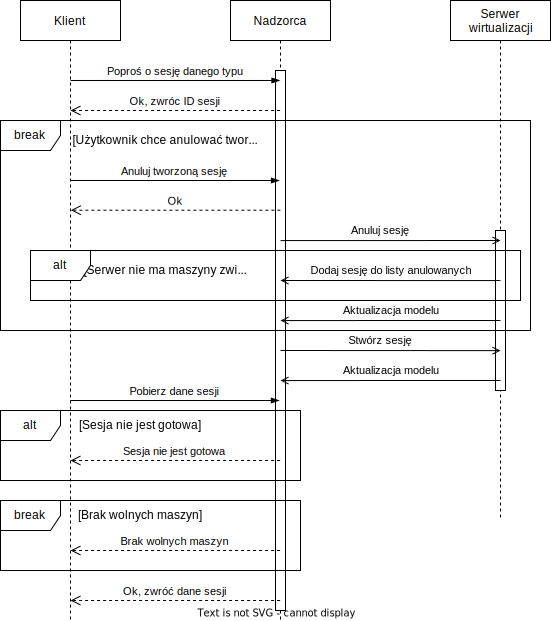
\includegraphics[width=\screenswidth]{sequence_diagrams/tworzenie_sesji.png}
	
	\vskip-1.5ex
	
	\caption{Diagram klas dla modelu systemu}
	\label{figure:diagrams:sequence_diagrams:tworzenie_sesji}
\end{figure}

Po prośbie użytkownika nadzorca znajduje wolna maszynę i prosi konkretny serwer wirtualizacji aby spróbował utworzyć sesje dla pewnego użytkownika.
Gdy to się uda, ten wysyła zbiorczą kolejką do nadzorców informacje o zmianie modelu.
W przeciwnym nadzorca powtarza prośbę.
O powtórzeniu zdecyduje otrzymany stan o danej maszynie (m.in. czy sesja do niej przypisana jest do tego użytkownika)

Może się zdarzyć także anulowanie wyszukiwania przez użytkownika.
Wtedy jeżeli maszyna jest już przydzielona użytkownikowi, to serwer wirtualizacji jest powiadamiany o anulowaniu sesji, aby ją anulował.
Jeżeli nie została jeszcze utworzona, to nadzorca dopilnuje aby więcej nie szukać sesji lub wyłączy ją w miarę potrzeby.

\pagebreak

\subsubsection{Zakończenie sesji}

Zdarzenie kończenia sesji oznacza powiadomienie konkretnego serwera wirtualnego aby wyłączył konkretną maszynę.
Serwer może odmówić z powodów różnic modelu. Wtedy wyśle tylko informacje o jego zmianie.

\begin{figure}[!h]
	
	\centering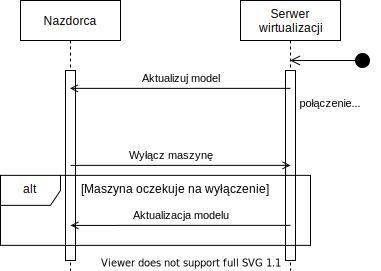
\includegraphics[width=\screenswidth]{sequence_diagrams/konczenie_sesji.png}
	
	\vskip-1.5ex
	
	\caption{Diagram klas dla modelu systemu}
	\label{figure:diagrams:sequence_diagrams:konczenie_sesji}
\end{figure}

\subsubsection{Aktualizacja stanu}

Nadzorca może w każdej chwili poprosić wszystkie serwery wirtualizacji
o aktualny stan ich części systemu poprzez wspólna kolejkę \hyperref[external-modules:broker:queue-virtsrv]{do serwerów wirtualizacji}.
Serwery muszą bezwarunkowo odpowiedzieć aktualnym stanem do wspólnej \hyperref[external-modules:broker:queue-overseers]{kolejki zwrotnej}.

\begin{figure}[!h]
	
	\centering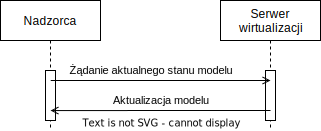
\includegraphics[width=\screenswidth]{sequence_diagrams/aktualizacja_stanu.png}
	
	\vskip-1.5ex
	
	\caption{Diagram klas dla modelu systemu}
	\label{figure:diagrams:sequence_diagrams:aktualizacja_stanu}
\end{figure}

\pagebreak

\subsubsection{Włączenie maszyny}

Nadzorca może poprosić konkretny serwer wirtualizacji aby utworzył maszynę o konkretnej nazwie.
Jeżeli maszynie nie istnieje, to zostanie uruchomiona oraz serwer odeśle powiadomienie \hyperref[external-modules:broker:queue-overseers]{zbiorcza kolejką} o zmianie modelu.
W przeciwnym wypadku nie zrobi nic.

\begin{figure}[!h]
	
	\centering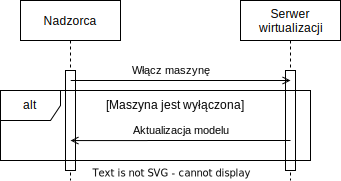
\includegraphics[width=\screenswidth]{sequence_diagrams/wlaczenie_maszyny.png}
	
	\vskip-1.5ex
	
	\caption{Diagram klas dla modelu systemu}
	\label{figure:diagrams:sequence_diagrams:wlaczenie_maszyny}
\end{figure}

\subsubsection{Wyłączenie maszyny}

Nadzorca może poprosić konkretny serwer wirtualizacji aby wyłączył konkretną maszynę wirtualną.
Jeżeli maszynę można wyłączyć to zostanie on wyłączona.
Następnie serwer wirtualizacji odeśle powiadomienie \hyperref[external-modules:broker:queue-overseers]{zbiorcza kolejką} o zmianie modelu.
W przeciwnym wypadku nie zrobi nic.

\begin{figure}[!h]
	
	\centering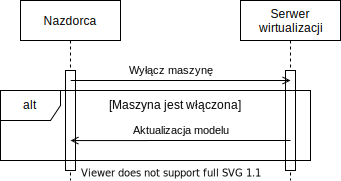
\includegraphics[width=\screenswidth]{sequence_diagrams/wylaczenie_maszyny.png}
	
	\vskip-1.5ex
	
	\caption{Diagram klas dla modelu systemu}
	\label{figure:diagrams:sequence_diagrams:wylaczenie_maszyny}
\end{figure}

\end{document}